%!TEX output_directory = build
%!TEX aux_directory = build


\documentclass[12pt]{article}
\usepackage{lingmacros}
\usepackage{tree-dvips}
\usepackage{amsmath}               
\usepackage{amsthm}
\usepackage{float}
\usepackage{multirow}
\usepackage{array}
\usepackage{subfigure}
\usepackage{afterpage}
\usepackage{amsmath,amssymb}            
\usepackage{rotating}  
\usepackage{fancyhdr}  
\usepackage{cancel}
\usepackage{tabularx}
\usepackage{multicol}
\usepackage{hyperref}
\usepackage{filecontents}
\usepackage{listings}
\usepackage{nomencl}
\usepackage{hyperref}
\usepackage{textcomp}
\usepackage{mathrsfs}
\usepackage{epigraph}
\usepackage[T1]{fontenc}
\usepackage[utf8]{inputenc}
\usepackage{xcolor}
%\usepackage[italian]{babel}
%\usepackage[latin1]{inputenc}
\usepackage[english]{babel}
\usepackage[nodisplayskipstretch]{setspace}
\setstretch{1.2}

\begin{document}

\newcommand{\fix}[1]{\textcolor{red}{FIX: #1} }   

\section*{Stability}

Once the NMPC problem has been formulated and the feasibility of the problem has been analyzed as in Equation \ref{feasibility} guaranteeing the fulfillment of hard  constraints, its stability has to be investigated. A proof of a terminal constraint-free approach for a nonlinear MPC is presented in \cite{alamir2018stability}. Anyway, parameterizing the control actions as in our approach, some considerations have to be done. \\
We will consider a zero-reference tracking problem considering the change of variables:
\begin{equation}\label{change_var}
    e_k=x_k-{x_d}_k
\end{equation}
and so, substituting \ref{change_var} in the state equation \ref{state_eq_param}, we can define:
\begin{equation} \label{NLsystem}
	\tilde{f}^+(e_{k|i}-{x_d}_k,p_k,t_i)-{x_d}_{k|i+1}=\hat{f}^+(e_{k|i},p_k,{{x_d}_{k|i}},{{x_d}_{k|i+1}},t_i) 
\end{equation}
then the discrete error state equation becomes:
\begin{equation}\label{sys_eq_con_e}
    e_{k|i+1}=\hat{f}^+(e_{k|i},p_k,{{x_d}_{k|i}},{{x_d}_{k|i+1}},t_i)=\hat{f}^+(e_{k|i},p_k,t_i)
\end{equation}
Note that, for simplicity of notation, the system equation in \ref{sys_eq_con_e} has been expressed as a function of the state error ${e_{k|i}}$ and the parameters $p_k$ only, given that the desired states are known.\\
In this way the problem is moved to track a zero error reference and becomes: 
\begin{equation} \label{ourproblem_stab}
\begin{split}
		& min_{{p}_k}\ J({e}_{k|0},{p}_k) =\sum_{i=1}^{N}\left(\frac{i}{N}\right)^b\hat{h}(e_{k|i},{p}_{k}) \\
		\textnormal{s.t.}\qquad
		&\ \ \ \ e_{k|i+1}=\hat{f}^+(e_{k|i},p_k,t_i) \\
		&\ \ \ \ e_{k|i} \in \mathbb{E}\ \forall\ i=1,\dots,\ N  \\
		&\ \ \ \ {p}_k\   \in \mathbb{P}\ \\
	\end{split}	
\end{equation}
where $\mathbb{E} = \lbrace {e}\in \mathbb{R}^n\ \textnormal{s.t.}\ {e}_{min}\leq e\leq e_{max} \rbrace$ is the feasible region of the state error and $\hat{h}$ is the stage cost function in \ref{costfunctionh} considering the change of variables in Equation \ref{change_var}. \\
Now, requiring that the point $e=0$ is a stable equilibrium point for the closed loop system means to establish that $J$ is a Lyapunov function, i.e. to assess that: 
\begin{equation}
	J({e}_{k+1|0},p^*_{k+1}) \leq J({e}_{k|0},p^*_k)
	\label{lyap_stab}
\end{equation}
Usually the most used approaches to verify this relies on a terminal constaint for the problem (i.e. $e_{k|N}=0$) or requiring the existence of a terminal set.
Anyway, the novelty of our approach lies in the absence of the terminal constraint and on the parameterization of the control action. Because of the latter, the extension of what done in \cite{alamir2018stability} is not straitforward and requires more general observations. \\
Given the optimal solution to the problem in \ref{ourproblem_stab} at time instant $k$ defined as $p_k^*=\left[ p_{k_1}^*,\ p_{k_2}^*,  \dots,\ p_{k_{N_p}}^* \right]^T$ that corresponds to $  \textbf{u}_k^*=[\ u_{k|0}^*,\ u_{k|1}^*,\  \dots,\  u_{k|{N-1}}^*\ ]$, consider the parameterization $\tilde{p}_{k+1}$ such that the correspondent control input is $  \tilde{\textbf{u}}_{k+1}=[\ u_{k|1}^*,\ u_{k|2}^*,\  \dots,\  u_{k|{N-1}}^*,\ \bar{u}_{k|N} \ ]$, where $\bar{u}_{k|N}$ does not belong to the optimal solution at time step $k$ but it is described with the same parameters. A clear graphical rapresentation of this can be seen in Figure \ref{param_translatability}. \fix{sarebbe da metter a posto questa immagine sotto}
\begin{figure}[h!]
	\centering
	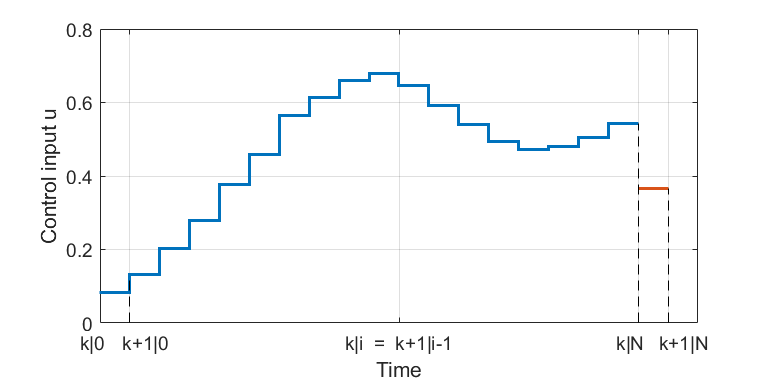
\includegraphics[scale=0.6]{IMMAGINI/trans_u.png}
	\caption{Translatability of the $F$ function}
	\label{param_translatability}
\end{figure}
The cost function generated from $\tilde{p}_{k+1}$ will be then:
\begin{equation}
	J({e}_{k+1|0},\tilde{p}_{k+1})=\sum_{i=1}^{N}\left(\frac{i}{N}\right)^b\hat{h}(e_{k+1|i},\tilde{p}_{k+1})
\end{equation}
which, for the definition of $\tilde{p}_{k+1}$, can be rewritten as:
\begin{equation}
\begin{split}
	J({e}_{k+1|0},\tilde{p}_{k+1})=J({e}_{k|0},p^*_k) -\left( \frac{1}{N} \right)^b\hat{h}(e_{k|1},p^*_{k}) + \hat{h}(\hat{f}^+(e_{k|N},p^*_k,t_N),p^*_k) \\
\end{split}
\end{equation}
Rearranging the terms:
\begin{equation}
\begin{split}
	\underbrace{J({e}_{k+1|0},\tilde{p}_{k+1})-J({e}_{k|0},p^*_k)}_{D}= \hat{h}(\hat{f}^+(e_{k|N},p^*_k,t_N),p^*_k) -\left( \frac{1}{N} \right)^b\hat{h}(e_{k|1},p^*_{k}) \\
\end{split}
\end{equation}
Verifying that the term $D$ is less than or equal to zero, means to assess the stability of the system because, for the definition of optimality of the solution, that also implies: $J({e}_{k+1|0},{p^*}_{k+1}) - J({e}_{k|0},{p^*}_k) \leq 0$, i.e. the relation in \ref{lyap_stab} holds. Therefore, $D\leq0$ admit a solution for any $k$, if 
\begin{equation}
\begin{split}
	\hat{h}(\hat{f}^+(e_{k|N},p^*_k,t_N))-\left( \frac{1}{N} \right)^b\hat{h}(e_{k|1},p^*_{k}) \leq 0 \\
\end{split}
\end{equation}
is always true for any $k$. Theoretically a value of $b$ for which the point $e=0$ is a stable equilibrium point for the closed loop system always exists, but it is not possible to define it precisely. This because it depends on the values of $\hat{h}(\cdot,\cdot)$; for example it is possible to have $\hat{h}(e_{k|1},p^*_{k})=0$ implying the need of $b=-\infty$ which is not practically possible.\\ The discussion is therefore reduced to the capacity of the solver decreasing the cost function with a parameterization $\tilde{p}_{k+1}$. This requirement, as shown in \cite{alamir_boh}, can be verified by looking at solving time and solver capabilities.

\end{document}